% C.15 直角△ 6,8,10 + 斜边高
\documentclass[tikz,border=4pt]{standalone}
\usepackage{ctex}
\usepackage{amsmath}
\usetikzlibrary{calc, arrows.meta}
\begin{document}
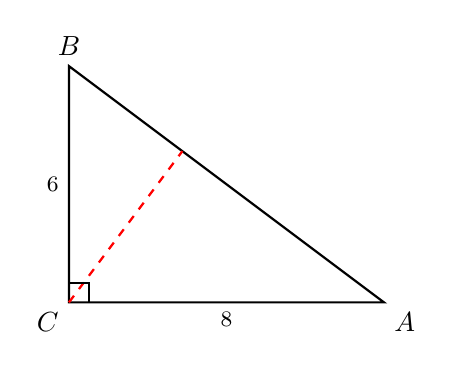
\begin{tikzpicture}[scale=0.5, thick]
  \coordinate (C) at (0,0);
  \coordinate (A) at (8,0);
  \coordinate (B) at (0,6);
  % foot of altitude from C to AB
  % AB direction (8,-6)/10; foot F = projection of C: F = A + ((C-A)·(B-A))/100 * (B-A)
  % (C-A)=(-8,0), (B-A)=(-8,6); dot = 64; t=64/100=0.64
  \pgfmathsetmacro{\fx}{8-0.64*8}
  \pgfmathsetmacro{\fy}{0.64*6}
  \coordinate (F) at (\fx,\fy);
  \draw (C) -- (A) -- (B) -- cycle;
  \draw[red, dashed] (C) -- (F);
  \draw (0,0.5) -- (0.5,0.5) -- (0.5,0);
  \node[below left] at (C) {$C$};
  \node[below right] at (A) {$A$};
  \node[above] at (B) {$B$};
  \node[font=\footnotesize, below] at (4,0) {$8$};
  \node[font=\footnotesize, left] at (0,3) {$6$};
\end{tikzpicture}
\end{document}
